% 25-cell taxonomy: 9 witness cells + 16 goal cells with verdict bits and labels.
% Designed for full text-width.
\begin{figure}[t]
\centering
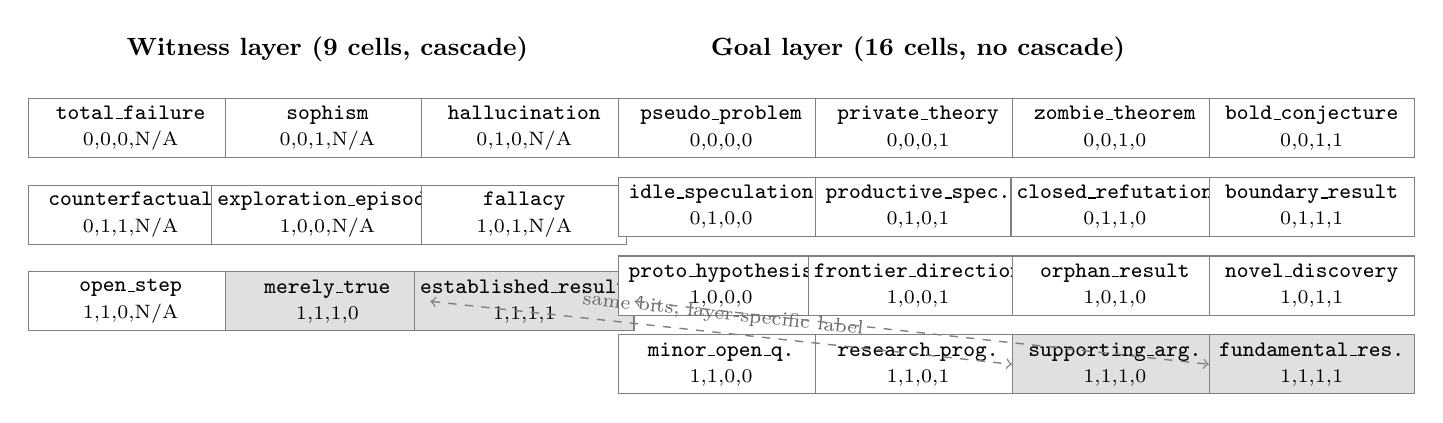
\begin{tikzpicture}[
  font=\footnotesize,
  cell/.style={
    rectangle, draw=black!50, fill=white,
    minimum width=2.6cm, minimum height=0.75cm, align=center,
    inner sep=2pt
  },
  cellgray/.style={
    cell, fill=black!12
  },
  bits/.style={font=\scriptsize\ttfamily, black!70},
  hdr/.style={font=\small\bfseries},
]

% Witness layer (left, 9 cells in a 3x3 grid + 2 highlighted bottom)
\node[hdr] at (-3.5, 4) {Witness layer (9 cells, cascade)};

\node[cell] (w1) at (-6, 3) {\texttt{total\_failure}\\{\scriptsize 0,0,0,N/A}};
\node[cell] (w2) at (-3.5, 3) {\texttt{sophism}\\{\scriptsize 0,0,1,N/A}};
\node[cell] (w3) at (-1, 3) {\texttt{hallucination}\\{\scriptsize 0,1,0,N/A}};
\node[cell] (w4) at (-6, 1.9) {\texttt{counterfactual}\\{\scriptsize 0,1,1,N/A}};
\node[cell] (w5) at (-3.5, 1.9) {\texttt{exploration\_episode}\\{\scriptsize 1,0,0,N/A}};
\node[cell] (w6) at (-1, 1.9) {\texttt{fallacy}\\{\scriptsize 1,0,1,N/A}};
\node[cell] (w7) at (-6, 0.8) {\texttt{open\_step}\\{\scriptsize 1,1,0,N/A}};
\node[cellgray] (w8) at (-3.5, 0.8) {\texttt{merely\_true}\\{\scriptsize 1,1,1,0}};
\node[cellgray] (w9) at (-1, 0.8) {\texttt{established\_result}\\{\scriptsize 1,1,1,1}};

% Goal layer (right, 16 cells in 4x4)
\node[hdr] at (4, 4) {Goal layer (16 cells, no cascade)};

\node[cell] (g1A) at (1.5, 3.0) {\texttt{pseudo\_problem}\\{\scriptsize 0,0,0,0}};
\node[cell] (g1B) at (4.0, 3.0) {\texttt{private\_theory}\\{\scriptsize 0,0,0,1}};
\node[cell] (g2A) at (6.5, 3.0) {\texttt{zombie\_theorem}\\{\scriptsize 0,0,1,0}};
\node[cell] (g2B) at (9.0, 3.0) {\texttt{bold\_conjecture}\\{\scriptsize 0,0,1,1}};

\node[cell] (g3A) at (1.5, 2.0) {\texttt{idle\_speculation}\\{\scriptsize 0,1,0,0}};
\node[cell] (g3B) at (4.0, 2.0) {\texttt{productive\_spec.}\\{\scriptsize 0,1,0,1}};
\node[cell] (g4A) at (6.5, 2.0) {\texttt{closed\_refutation}\\{\scriptsize 0,1,1,0}};
\node[cell] (g4B) at (9.0, 2.0) {\texttt{boundary\_result}\\{\scriptsize 0,1,1,1}};

\node[cell] (g5A) at (1.5, 1.0) {\texttt{proto\_hypothesis}\\{\scriptsize 1,0,0,0}};
\node[cell] (g5B) at (4.0, 1.0) {\texttt{frontier\_direction}\\{\scriptsize 1,0,0,1}};
\node[cell] (g6A) at (6.5, 1.0) {\texttt{orphan\_result}\\{\scriptsize 1,0,1,0}};
\node[cell] (g6B) at (9.0, 1.0) {\texttt{novel\_discovery}\\{\scriptsize 1,0,1,1}};

\node[cell] (g7A) at (1.5, 0.0) {\texttt{minor\_open\_q.}\\{\scriptsize 1,1,0,0}};
\node[cell] (g7B) at (4.0, 0.0) {\texttt{research\_prog.}\\{\scriptsize 1,1,0,1}};
\node[cellgray] (g8) at (6.5, 0.0) {\texttt{supporting\_arg.}\\{\scriptsize 1,1,1,0}};
\node[cellgray] (g9) at (9.0, 0.0) {\texttt{fundamental\_res.}\\{\scriptsize 1,1,1,1}};

% Specialization annotation between layers
\draw[<->, dashed, black!50, line width=0.5pt]
  (w8.east) -- node[font=\scriptsize, midway, above, sloped, black!60]
    {same bits, layer-specific label} (g8.west);
\draw[<->, dashed, black!50, line width=0.5pt]
  (w9.east) -- node[font=\scriptsize, midway, above, sloped, black!60]
    {} (g9.west);

\end{tikzpicture}
\caption{The locked verdict-bits to cell-label assembly mapping. Witness layer
(left, 9 cells): cascade collapses 7 of 16 verdict vectors to $\text{Inv}=\text{N/A}$;
the remaining 9 cells are named by the witness-layer interpretation of each
gate. Goal layer (right, 16 cells): all four gates fire independently, so
the full $2^4$ verdict space is named.
The two cells highlighted in each layer share verdict bits with their counterparts
in the other layer (the dashed two-headed arrows): $(1,1,1,0)$ is
\texttt{merely\_true} as a witness but \texttt{supporting\_argument} as a goal;
$(1,1,1,1)$ is \texttt{established\_result} as a witness but
\texttt{fundamental\_result} as a goal. This is specialization-at-instance,
not a violation of gate-invariance.}
\label{fig:cell_taxonomy}
\end{figure}
